\documentclass{article}
\usepackage[utf8]{inputenc}
\usepackage[russian]{babel}   % Подключение модуля для русского языка
\title{Конспект лекций И.А. Халидова по Теории Функции Комплексной переменной}
\author{Григорий Ефимов}
\date{Сентябрь - Декабрь 2021}
\usepackage{mathtools}
\usepackage{graphicx}
\usepackage{amssymb}
\usepackage{float}
\graphicspath{{img/}}
\DeclareGraphicsExtensions{.pdf,.png,.jpg}
\begin{document}
    \begin{titlepage}
      \maketitle
    \end{titlepage}
    \tableofcontents
    \newpage
    \section{Введение}
        \subsection{Литература}
            \begin{itemize}
                \item Аксенов ТФКП
                \item Волькер Задачник
            \end{itemize}
            \newpage
        \subsection{Как устроены комплексные числа}
            \begin{equation}\label{eq:algebraik_form_complex}
                z=x+iy\footnotemark
            \end{equation}
            \footnotetext{ $i=-1$ }
            \begin{equation}\label{eq:algebraik_form_complex_w}
                w=u+iv
            \end{equation}
            Формула \ref{eq:algebraik_form_complex} - представление комплексного числа в алгебраическом виде. $x=Re(z)$ - вещественная часть комплексного числа (англ. real) $y=Im(z)$ - мнимая часть комплексного числа (англ. imagine)\\
            \begin{equation}\label{eq:exponential_form_complex}
                z=re^{i\phi}
            \end{equation}
            \begin{equation}\label{eq:trigonometric_form_complex}
                z=r(cos(\phi)+i sin(\phi))
            \end{equation}
          Формула \ref{eq:exponential_form_complex} - представление комплексного числа в показательной, формула         \ref{eq:trigonometric_form_complex} - в тригонометрической форме.\\
            Z \footnote{Часто множество комплексных чисел обозначают $C$, но мы так делать не будем, так как это обозначение сопадает с множеством непрерывных функкций} - множество комплексных чисел, т.е. комплексная плоскость. Если задаётся несколько плоскостей, то вторая задаётся буквой W и форумула \ref{eq:algebraik_form_complex_w} соответственно.
            \begin{equation}\label{eq:сomplex_module}
                |z|=sqrt(x^2+y^2)
            \end{equation}
            Модуль комплексного числа определяется по формуле \ref{eq:сomplex_module}
            \begin{figure}[h]
                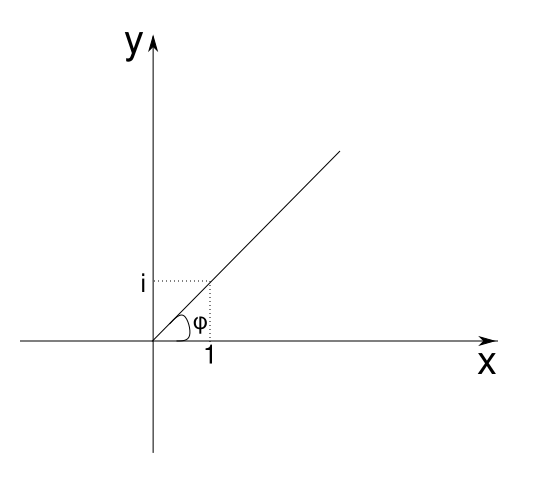
\includegraphics[width=0.6\linewidth]{complex_example}
                \caption{Графическое представление комплексного числа}
                \label{ris:complex_example}
            \end{figure}
              \begin{equation}\label{eq:complex_polar_example_x}
                  |z|cos(\phi)=x
              \end{equation}
              \begin{equation}\label{eq:complex_polar_example_y}
                  |z|sin(\phi)=y
              \end{equation}
            Формулы \ref{eq:complex_polar_example_x} и \ref{eq:complex_polar_example_y} нужны для представления полярного угла, являющегося $arg(z) $
            при этом важно, что $arg(z) \neq arctg(y/x)$, т.к. это корректно только для положительной полуплоскости
            \begin{equation}\label{eq:Arg_z}
                Arg(z)=\phi+2 \pi n
            \end{equation}
            Формуле \ref{eq:Arg_z} - формула аргумента уомплексного числа, т.е. множества чисел, отстоящих друг от дргуа на $2 \pi$, важно что Arg пишется с большой буквы. $arg(z)$ - главное значение аргумента, 
            \begin{math} 
              arg(z) \in 
              \begin{cases}
                [0;2 \pi] ($по учебнику$)\\
                [-\pi;\pi] ($этот вариант предпочтительней \footnotemark $)
              \end{cases} 
            \end{math}\\
            \footnotetext{Удобнее работать с чётностью, разрыв z будет в отрицательной полуплоскости, а в ней работают в реальных задачах реже}
            Комплексные числа работают с алгебраическими операциями и сохраняют свойства ассоциативности, дистрибутивности и комутативности.\\
            \begin{equation}\label{eq:Arg_z}
                z_{1} \pm z_{2}=(x_{1} \pm x_{2}) + i (y_{1} \pm y_{2})
            \end{equation}
          Сложение комплексных чисел в алгебраической форме\footnote{В полярной системе складывать комплексные числа сложнее сложнее}
            \begin{figure}[h]
                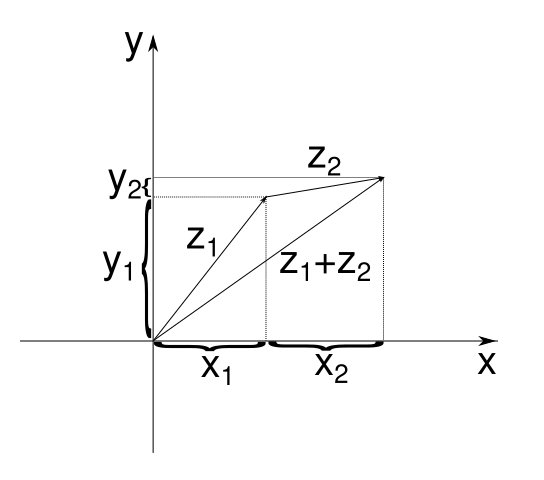
\includegraphics[width=0.8\linewidth]{adding_example}
                \caption{Графическое представление сложения двух комплексных чисел}
                \label{ris:adding_example}
            \end{figure}
            \begin{equation}
               z_{1} \cdot z_{2}=r_{1} r_{2} e^{i (\phi_{1} + \phi_{2})}              
            \end{equation}
            Уножение комплексных чисел в показательной форме\footnote{Для умножения удобнее использовать показательную, а не албебраическую форму}. Аналогично и с делением:
            \begin{equation}
               \frac{z_{1}}{z_{2}}=\frac{r_{1}}{r_{2}} e^{i (\phi_{1} - \phi_{2})}              
            \end{equation}
          Возведение в степень:
            \begin{equation}
               z=r^{n} e^{i n \phi}              
            \end{equation}
            $ \overline{z} $, иногда $z^{*}$ - комплексно-сопряженное число\footnote{Точка отражается относитеьно вещественной оси}, определим z из формулы \ref{eq:algebraik_form_complex}, тогда:
            \begin{equation}\label{complex_conjugate}
               \overline{z}=x-i y              
            \end{equation}
            \begin{equation}\label{complex_conjugate}
               \overline{z_{1} \pm z_{2}}=\overline{z_{1}} \pm \overline{z_{2}}              
            \end{equation}
            \begin{equation}\label{complex_conjugate}
               \overline{z_{1} \cdot z_{2}}=\overline{z_{1}} \cdot \overline{z_{2}}              
            \end{equation}
            С помощью комплексно-сопряжённых чисел можно делить комплексные числа в алгебраической форме:
            \begin{equation}
               \frac{ z_{2} }{ z_{1} } = \frac{ z_{2} \cdot \overline{ z_{1} }}{ \overline{z_{1}} \cdot z_{1} }
            \end{equation}
            \begin{equation}
               z \cdot \overline{z}=|z^{2}|
            \end{equation}
          Извлечение корня n степени из комплексного числа\footnote{Важно что Arg(z) - с большой буквы, т.к. значение не одно}, $n \in N $
            \begin{equation}
              \sqrt[n]{z}=\sqrt[n]{r} e^{\frac{i}{n} Arg(z)}=\sqrt[n]{r} e^{\frac{i}{n} \phi + 2 \pi k}
            \end{equation}
          Получается n корней, т.к. $\frac{2 \pi k}{n}$ имеет период n, и значения начнут повторяться. В точке 0 и в $\infty$ \footnote{
              В вещественных числах существует $+ \infty$ и $- \infty$, а у комплексных чисел есть только z=$\infty$, в неё можно попасть любым путём.
            } аргумент не определён
            \newpage
        \section{Стереографическая проекция}
        \subsection{Стереографическая проекция}
            \begin{figure}[h]
                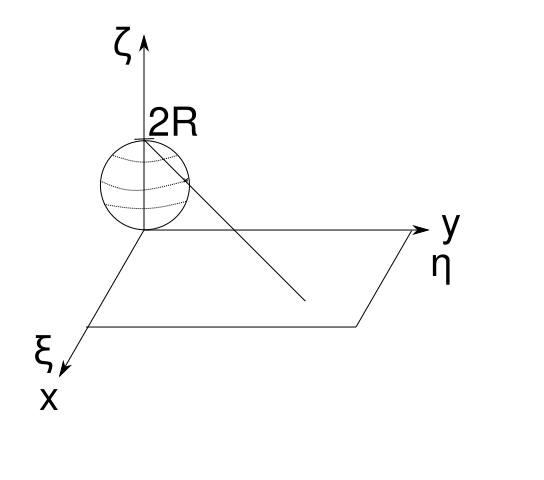
\includegraphics[width=0.8\linewidth]{stereo_example}
                \caption{Стереографическая проекция на сфере Римана}
                \label{ris:stereo_example}
            \end{figure}
            $X o Y$ - комлексная плосокость. Переобозначим в трёхмерной плоскости. Построим сферу радиусом R \footnote{Чаще всего радиус задают как R=$\frac{1}{2}$ , однако, он может быть любым} с центром в точке (0,0,R). Сопоставим каждую точку на комплескной плоскости с точкой на сфере. Для этого проведём прямую из верхней точки сферы (0,0,2R) в точку z на XoY, точка, в которой прямая пересекает сферу - отображениие точки z на сфере. $z=0 \Leftrightarrow (\xi,\zeta,\eta)=\varnothing$ . Аналогично любая точка сферы кроме (0,0,2R) \footnote{$z=0 \Leftrightarrow (\xi,\zeta,\eta)=(0,0,2R)$} может быть сопоставлена с точкой на комплексной плоскости. Для этого из точки (0,0,2R) проводится прямая, проходящая через заданную точку сферы. Точка, в которой прямая пересекает комплексную плоскость, будет отображанием.\\
          Формулы для перевода координат:
            \begin{math}
              (0,0,2R),(x,y,0) - $ точки прямой, тогда уравнение этой прямой имеет вид: $\\
              \frac{\xi-0}{x-0}=\frac{\eta-0}{y-0}=\frac{\zeta-2R}{0-2R}\\
            $ Уравнение сферы с центром в (0,0,2R) и радиусом R: $\\
              \xi^{2}+\eta^{2}+(\zeta-R)^{2}=R^{2}\\
            $ Получаем систему: $
              \begin{cases}
                \frac{\xi}{x}=\frac{\eta}{y}=\frac{\zeta-2R}{-2R}\\
                \xi^{2}+\eta^{2}+(\zeta-R)^{2}=R^{2}
              \end{cases}\\
            $ Решение системы: $
              \begin{cases}
                \xi=\frac{4R^{2}x}{x^{2}+y^{2}+4R^{2}}\\
                \eta=\frac{4R^{2}y}{x^{2}+y^{2}+4R^{2}}\\
                \zeta=\frac{2R(x^{2}+y^{2})}{x^{2}+y^{2}+4R^{2}}\\
              \end{cases}\\ $В обратную сторону: $ 
              \begin{cases}
                x=\frac{2R \xi}{2R-\zeta}\\
                x=\frac{2R \eta}{2R-\zeta}\\
              \end{cases}
            \end{math}
            \newpage
          \section{Примеры решения неравенств с комплексными числами}
          \subsection{Пример 1}
          \begin{math}
            |1+z^{2}|<|2z|\\
            1+z^{2}=1+x^{2}-y^{2}+i 2 x y\\
            2z=2x+i 2y\\
            \sqrt{(1+x^{2}-y^{2})^{2}+(2 x y)^{2}} < \sqrt{(2x)^{2}+(2 y)^{2}} \Rightarrow\\
            (1+x^{2}-y^{2})^{2}+(2 x y)^{2} < (2x)^{2}+(2 y)^{2}\\
            (1+x^{2}-y^{2})^{2}+4 x^{2} y^{2} < 4x^{2}+4y^{2}\\
            4 x^2 y^2 + 2 x^2 - 4 y + 2<4 x^2 + 4 y^2\\
          $Получаем$ (1-x^{2}-y^{2})^{2}<4y^{2}\\
          $Рассмотрим случай $y>0 $ : $\\
            -2y<1-x^2-y^y\\
          $Получаем два неравенства:$\\
          \end{math}
          \begin{enumerate}
            \item  $x^2+y^2-2y+1<2$
            \item  $x^2+y^2+2y+1>2$
          \end{enumerate}

        Получаем уравнения двух окружностей, решением является то, что находится внутри первой окржности и одновременно снаружи второй, т.е. A$ \backslash $B. Аналогично будет для $y<0$, из уравнений получатся те же две окружности, но решением будет B$ \backslash $A.
        Решением всей хадачи будет (A$ \backslash $B) $\cup$ (B$ \backslash $A)
         \begin{figure}[h]
            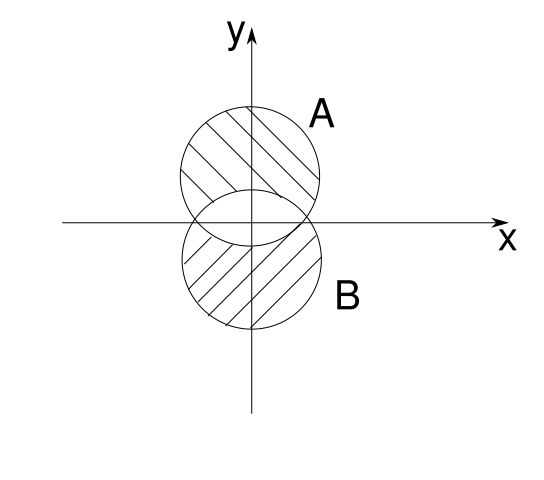
\includegraphics[width=0.6\linewidth]{complex_solution_example}
            \caption{Решение неравенства $|1+z^{2}|<|2z|$}
            \label{ris:complex_solution_example}
         \end{figure}
         \section{Функция комплексной переменной}
            \subsection{Предел}
                \begin{figure}[h]
                  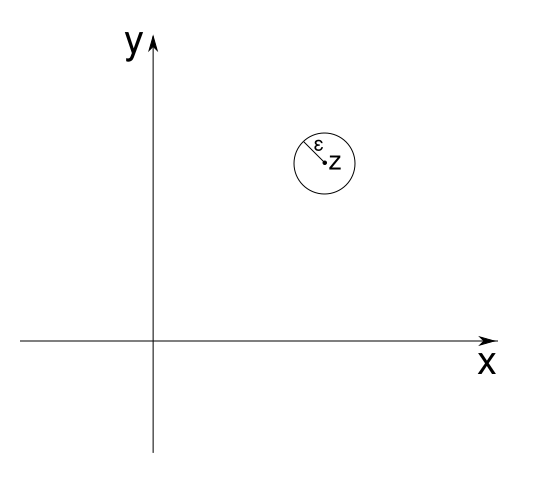
\includegraphics[width=0.6\linewidth]{complex_epsilon_example}
                  \caption{Эпсилон-окрестность точки z}
                  \label{ris:complex_epsolon_example}
                \end{figure}
                $\forall \epsilon > 0 \exists N : \forall n>N $ : 
                $|z_{n}-z|< \epsilon$\\
             Для функции двух переменных предел отдельно для каждой переменной $ z_{n} \rightarrow z,n \rightarrow \infty \Leftrightarrow x_{n} \rightarrow x,y_{n} \rightarrow y$\\
             А для функции комлпексной переменной\\ \begin{math} \begin{cases} x_{n} \rightarrow x \\ y_{n} \rightarrow y \end{cases} \Rightarrow 
             \begin{cases} r_{n} \rightarrow r \\ \phi_{n} \rightarrow \phi \end{cases} \end{math}
              , \begin{nobreak} $\phi \neq 0$, $\phi \neq \infty$ \end{nobreak} 
              \newpage
           \subsection{Комплексная функция с вещественным аргументом}
             $ t \in R $ , $z \in Z z=f(t) \Rightarrow \begin{cases} x(t)\\y(t) \end{cases} $ - кривая на плоскости \footnote{в данном случае на комплексной}.\\
             $f(t)$ непрерывная, дифференцируема, есди $x(t)$ и $y(t)$ непрерывны и дифференцируемы.\\
             \begin{figure}[H]
                  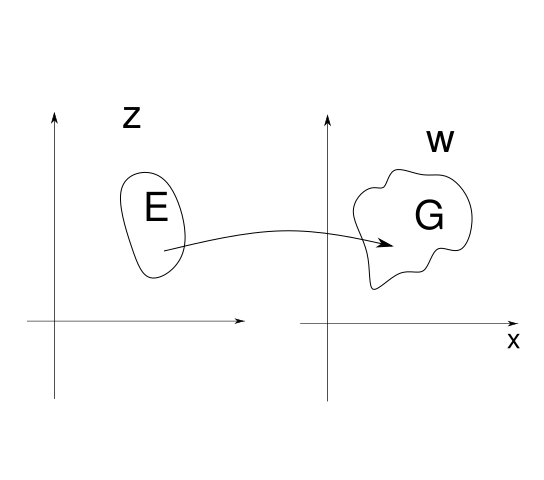
\includegraphics[width=0.6\linewidth]{complex_imagine_example}
                  \caption{Отображение значений комплексной функции}
                  \label{ris:complex_imagine_example}
              \end{figure}
         Функция определена на плоскости если кажой точке e в E\footnote{Области определения функции} соответствует точка g в G\footnote{ Области допустисых значений}.\\ Задать функцию комплексной переменной $\Leftrightarrow$ задать $u(x,y)$ и $v(x,y)$ вещественных функций от комплексного аргумента.\\
         Предел для функции комплексной переменной аналогичен пределу для функции нескольких переменных
           \begin{enumerate}
             \item $A=lim(f(z))$\\
             $z \rightarrow z_{0} \forall \epsilon>0 \exists \delta>0 \forall z \in U _{ \delta }(z_{0} \cap E)$ : $|A-f(z)|< \epsilon$
             \item $A=\infty$ \\
             $\forall \epsilon>0 \exists \delta>0 \forall z \in U _{ \delta }(z_{0} \cap E)$ :$ U_{\epsilon}(\infty) \Leftrightarrow |f(z)|< \frac{1}{\epsilon}$
           \end{enumerate}
            \begin{figure}[H]
                  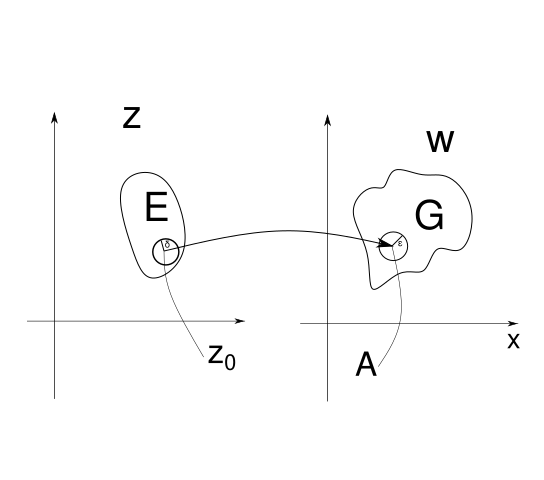
\includegraphics[width=0.6\linewidth]{complex_imagine_example2}
                  \caption{Отображение значений комплексной функции в окрестности точки}
                  \label{ris:complex_imagine_example2}
            \end{figure}
            Функция непрерывна в $z_{0}$, если $\exists lim_{z \rightarrow z_{0}}$, $z \in E$\\
            Непрерывность в $\infty$, если существует $lim_{z \rightarrow \infty} f(z)$, доопределяют функцию f(z), говоря что в точке $\infty f(z)=A$. Равномерная непрерывность отличается от непрерывности тем, что $\delta$ одинаковый для предела во всех точках множества $E$.
            \newpage
            \subsection{Теорема Кантора}
            Функция непрерывна на компактном\footnote{замкнутом} множестве является равномерно непрерывной
\end{document} 
